% Author: Ben Liao, Jason Zhang, Olivia Huang, Sylvia Jin

\qns{Minimum Norm Solution \& Pseudoinverse}

The Moore-Penrose Pseudoinverse is essentially a way to calculate "inverses" of \textbf{wide matrices}. The cardinal problem of linear algebra is solving the problem $A\vec{x} = \vec{b}$. If $A$ is square, we can use Gaussian elimination to solve the problem. If $A$ is tall, the system is overdetermined (i.e. more equations than unknowns), and we can use Least Squares to find the solution that minimizes the error, i.e. the quantity $\lVert A\vec{x} - \vec{b} \rVert$. If $A$ is wide, the system is underdetermined (i.e. fewer equations than unknowns), so there are infinitely many solutions to the system (infinitely many $\vec{x}$ that solve the equation). So, which solution is the "best" one? In many situations, we want to choose the solution that has the \textbf{smallest norm}. It's useful to think of this as the "shortest vector" that satisfies the equation.

The point: given a wide matrix $A$ and a vector $\vec{b}$ in the output space of $A$, the Moore-Penrose Pseudoinverse $A^\dagger$ gives the "smallest/shortest" solution vector $\vec{x}$ as $\vec{x} = A^\dagger \vec{b}$, such that $A\vec{x} = \vec{b}$. And this is guaranteed!

\begin{enumerate}
	%% part a
  	\qitem Suppose we have the matrix
  		\begin{equation*}
    		A = \begin{bmatrix} 1 & 2 \end{bmatrix}
    	\end{equation*}
    	and $b = 2$ and we want to solve the system $A\vec{x} = b$. Find some vectors $\vec{x}$ that solve this equation.

    \meta{
    	Mention that this is basically trying to find $x_1$, $x_2$ that solves $1x_1 + 2x_2 = 2$. Students probably won't need that information to solve the problem, but it's useful for building intuition in later parts.
    }
  	
	\ws{
    	\vspace{100px}
  	}
  
  	\sol {
    	Some possible solutions for $x$ are: $\begin{bmatrix} 0 \\ 1 \end{bmatrix}$, $\begin{bmatrix} 2 \\ 0 \end{bmatrix}$, $\begin{bmatrix} 1 \\ 0.5 \end{bmatrix}$, $\begin{bmatrix} 4 \\ -1 \end{bmatrix}$.
  	}

  %% part b
  \qitem Find the norms of the vectors you found in part a). Which one has the smallest norm?

  \ws{
    \vspace{100px}
  }

  \sol {
    Answer is based on part a). Graphically, it is the shortest length vector.
  }

  %% part c
  \qitem Plot the vectors you found in part a). Do you notice any patterns? Where do all the solutions lie?

  \ws{
    \begin{figure}[H]
    \centering
    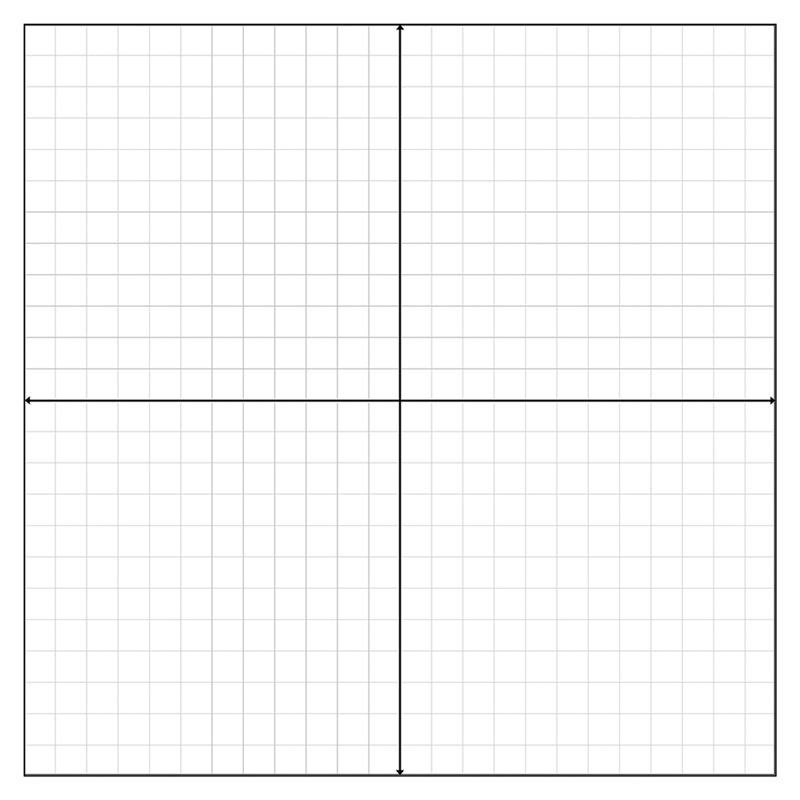
\includegraphics[width=.5\textwidth]{\bank/min-norm/figures/plane_blank.jpg}
    \end{figure}
  }

  \sol {
    The line consisting of points $a\begin{bmatrix} -2 \\ 1 \end{bmatrix} + \begin{bmatrix} \frac{2}{5} \\ \frac{4}{5} \end{bmatrix}$ for $a \in \mathbb{R}$.
    \begin{figure}[H]
    \centering
    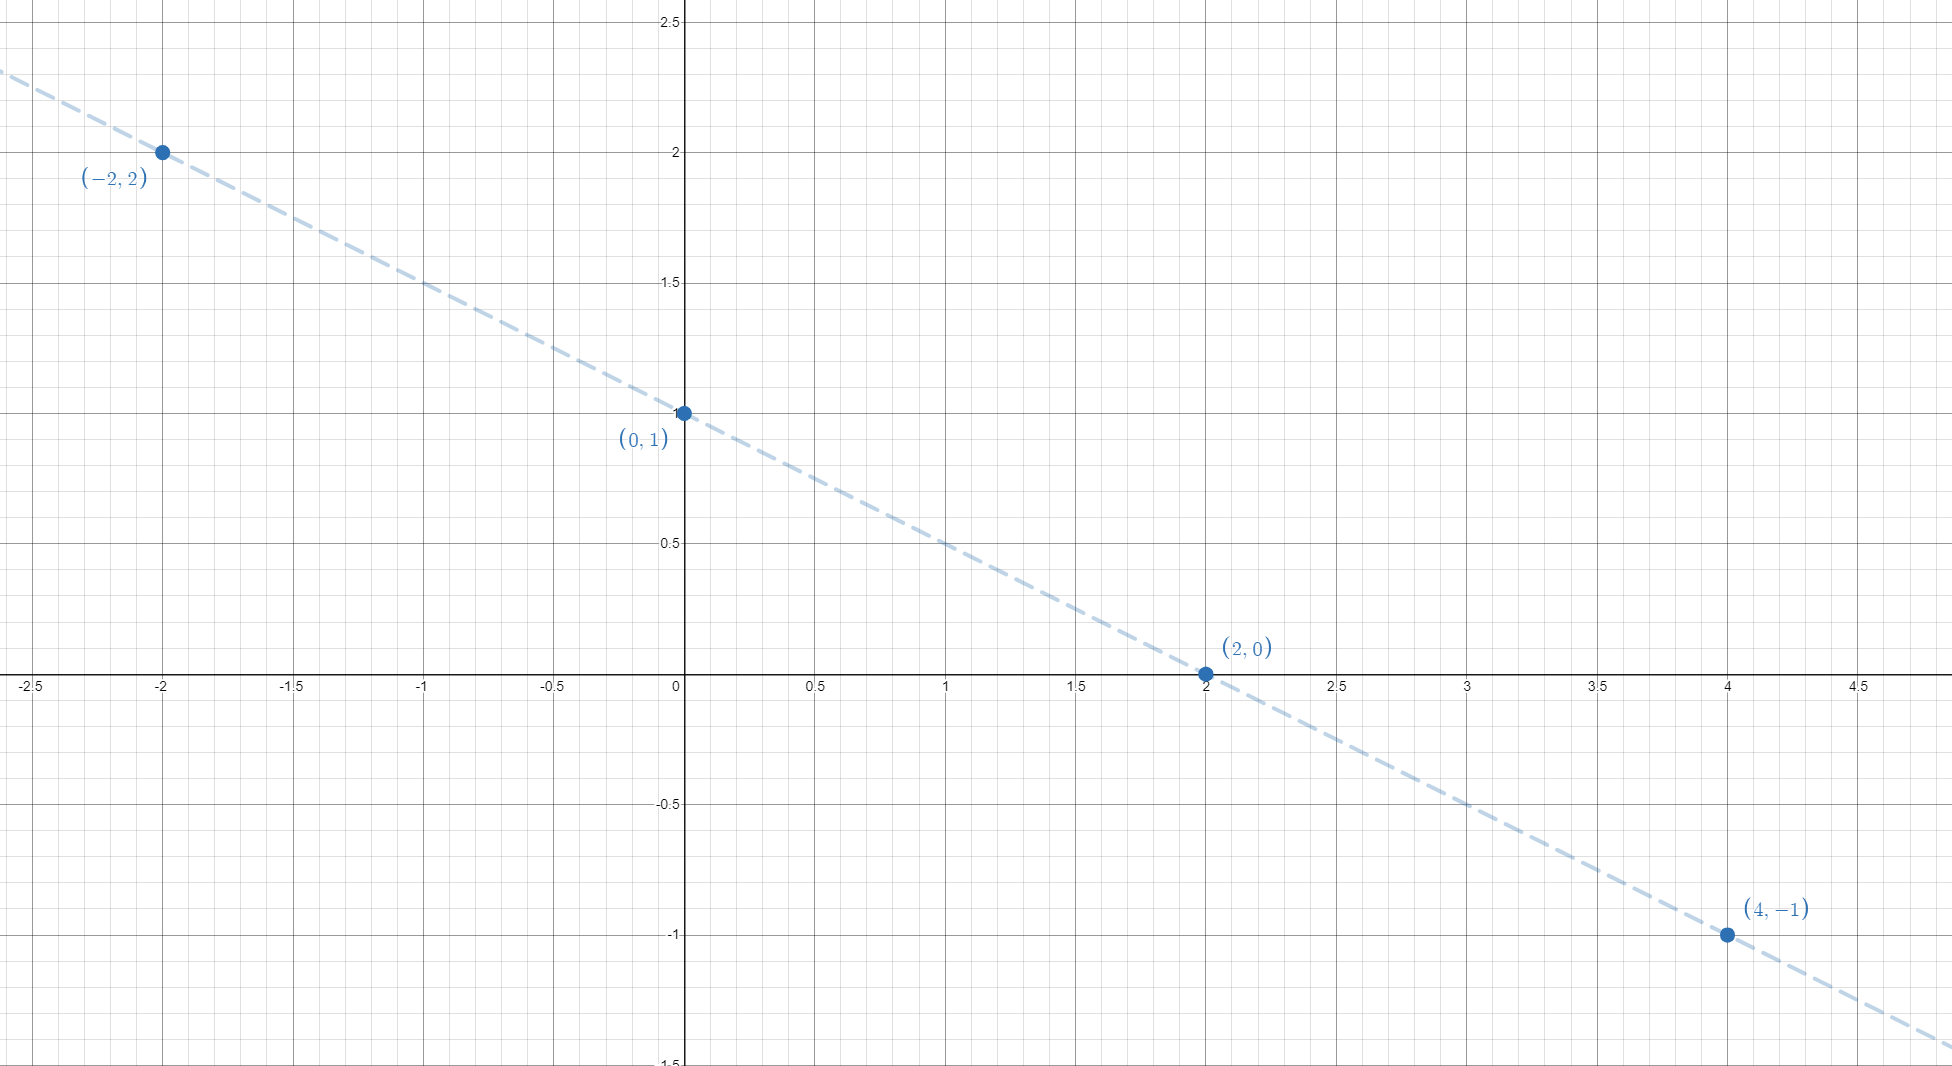
\includegraphics[width=0.9\textwidth]{\bank/min-norm/figures/sol_c.png}
    \end{figure}
  }

  %% part d
  \qitem Geometrically, what is the minimum norm solution to the problem? (\textit{Hint:} Which vector among the solutions to the problem has the shortest length?)
  
  \meta{
  	Make sure to mention to students why this particular solution is the shortest one. You can think of any other solution (which will lie on the blue dotted line) as the red solution \textit{plus} some component along the blue line. But the component along the blue line doesn't help the solve the problem in some sense, all it does is add length to the solution vector. The vector that "solves the problem without wasting any energy" is the $\begin{bmatrix} \frac{2}{5} \\ \frac{4}{5} \end{bmatrix}$ vector. We try to prove this in general in parts h) and i).
  }
  \ws{
    \vspace{100px}
  }

  \sol {
    The minimum norm solution is perpendicular to the line of solutions. To find the numerical solution, you might find the equation of the line that passes through the origin and intersects the line of solutions at a perpendicular angle. This is the line $y = 2x$. The vector along that line that reaches the line of solutions is $\begin{bmatrix} \frac{2}{5} \\ \frac{4}{5} \end{bmatrix}$.
    \begin{figure}[H]
    \centering
    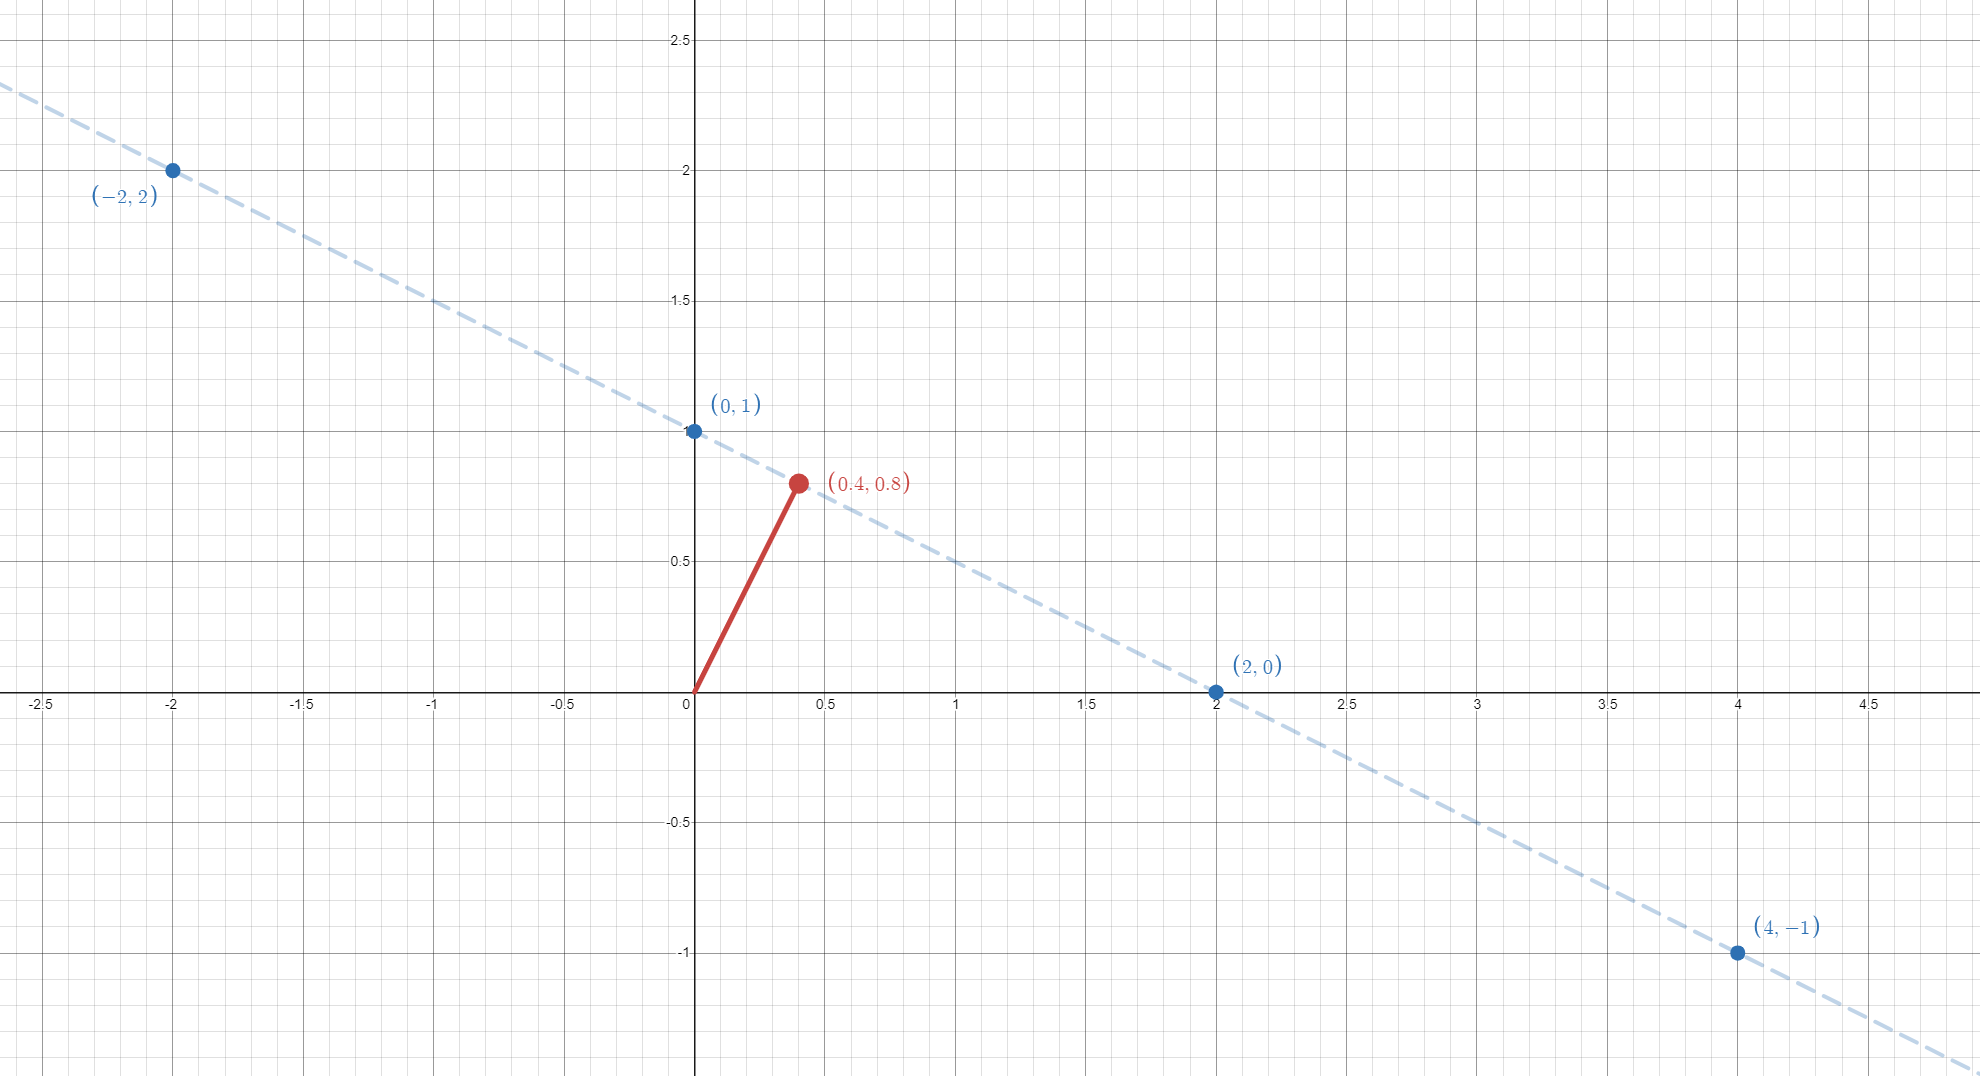
\includegraphics[width=0.9\textwidth]{\bank/min-norm/figures/sol_d.png}
    \end{figure}
  }

  %% part e
  \qitem Now, find the nullspace of $A$. i.e. find the set of $\vec{x}$ such that $A\vec{x} = 0$.
  \meta{
  	Make sure students notice that this null space corresponds exactly to all the vectors you can add to the optimal solution found in part d) to obtain additional solutions to the original problem.
  }
  \ws{
    \vspace{100px}
  }

  \sol {
    Null($A$) = Span$\Bigg\{ \begin{bmatrix} -2 \\ 1 \end{bmatrix}\Bigg\}$
  }

  %% part f
  \qitem Calculate the full SVD of $A$.

  \ws{
    \vspace{200px}
  }

  \sol {
    Step 1: A is a wide matrix, so we use $AA^T$: $AA^T = \begin{bmatrix} 1 & 2 \end{bmatrix}\begin{bmatrix} 1 \\ 2 \end{bmatrix} = \begin{bmatrix} 5 \end{bmatrix}.$ 
	
    Step 2: Find the eigenvalue(s) and corresponding eigenvector(s) of $AA^T$.
	
    \indent\indent By inspection, $\lambda = 5$ and $\vec{u} = \begin{bmatrix} 1 \end{bmatrix}$.
	
    Step 3: Compute the singular value(s): $\sigma = \sqrt{\lambda} = \sqrt{5}$
	
    Step 4: Compute the vector $\vec{v}$ using the formula:
    $$
    \vec{v_1} = \frac{A^T \vec{u}}{\sigma} = 
    \frac{\begin{bmatrix} 1 \\ 2 \end{bmatrix}\begin{bmatrix} 1 \end{bmatrix}}{\sqrt{5}}
    =  \begin{bmatrix} \frac{1}{\sqrt{5}} \\ \frac{2}{\sqrt{5}} \end{bmatrix}
    $$
    
    Step 5: Compute the second vector $\vec{v_2}$ in the $V$ matrix. Remember that it must be orthogonal to $\vec{v_1}$:
    $$ \vec{v_2} = \begin{bmatrix} - \frac{2}{\sqrt{5}} \\ \frac{1}{\sqrt{5}} \end{bmatrix} $$ \newline
	
    You can check to see that this vector is indeed orthogonal to $\vec{v_1}$ by verifying that $\vec{v_1} \cdot \vec{v_2} = 0$
    
    So now we have our SVD, which is:
    $$
    A = \begin{bmatrix} 1 & 2 \end{bmatrix} = 
    \begin{bmatrix} 1 \end{bmatrix} \begin{bmatrix} \sqrt{5} & 0 \end{bmatrix} 
    \begin{bmatrix} \frac{1}{\sqrt{5}} & \frac{2}{\sqrt{5}} \\ -\frac{2}{\sqrt{5}} & \frac{1}{\sqrt{5}} \end{bmatrix} = U \Sigma V^T
    $$
  }
  
  %% part g
  \qitem Write out the pseudoinverse $A^\dagger = V\tilde{\Sigma}U^T$. Then calculate the minimum norm solution as $\vec{x} = A^\dagger b$. Is it the same as what we determined geometrically?
  
  \meta{
  	Remind students that we are looking to solve $Ax = b$. Normally, we can use $x = A^{-1}b$. Note its similarity to $x = A^{\dagger}b$.
  }
  
  \ws{
  	\vspace{100px}
  }
  
  \sol{
    \begin{align*}
    A^\dagger &= \begin{bmatrix} \frac{1}{\sqrt{5}} & \frac{2}{\sqrt{5}} \\ 
    -\frac{2}{\sqrt{5}} & \frac{1}{\sqrt{5}} \end{bmatrix} \begin{bmatrix} \frac{1}{\sqrt{5}} \\ 
    0 \end{bmatrix} \begin{bmatrix} 1 \end{bmatrix} = V  \tilde{\Sigma} U^T \\
    A^\dagger &= \begin{bmatrix} \frac{1}{5} \\ \frac{2}{5} \end{bmatrix}
    \end{align*}
    
    Then calculating $\vec{x} = A^\dagger b$ gives:
    \begin{align*}
        A^\dagger b = \begin{bmatrix} \frac{1}{5} \\ \frac{2}{5} \end{bmatrix} \cdot 2 = \begin{bmatrix} \frac{2}{5} \\ \frac{4}{5} \end{bmatrix}
    \end{align*}
    which matches what we found geometrically in part d).
  }
  
  %% part h
  \qitem Show that if $\vec{x}^*$ is a solution to $A\vec{x} = \vec{b}$, then $\vec{x}^* + \vec{n}$ is also a solution to $A\vec{x} = \vec{b}$ for $\vec{n}$ in the nullspace of $A$.
  
  \meta{
  	Mention that the nullspace of $A$ says something about the ``dimension'' of the set of solutions to $Ax = b$. Ex. if $A$ is a super wide matrix, then the nullspace of $A$ will have higher dimension, and so the set of solutions to $Ax = b$ will be large.
  }
  
  \ws{
  	\vspace{100 px}
  }
  
  \sol{
  	For all $n \in N(A)$, $A(x^* + n) = Ax^* + An = Ax^* = b$.
  }
  
  %% part i
  \qitem Show that if $\vec{x}^*$ is orthogonal to the nullspace, then the norm of $\vec{x}^*$ is less than the norm of all $\vec{x}^* + \vec{n}$ for $\vec{n}$ in the nullspace of $A$.
  
  \ws{
  	\vspace{100px}
  }
  
  \sol{
    For all vectors $x^* + n$ in the set of solutions to $Ax = b$, 
    \begin{align*}
        \lVert x^* + n\rVert^2 &= \langle x^* + n, x^* + n \rangle \\
        &= \langle x^*, x^* \rangle + \langle x^*, n \rangle + \langle n, x^* \rangle + \langle n, n \rangle \\
        &= \lVert x^* \rVert ^2 + \lVert n \rVert ^2 \\
        & \geq \lVert x^* \rVert ^2
    \end{align*}
    So $x^*$ has smallest norm.
  }
  
\end{enumerate}
